\documentclass[11pt,a4paper]{article}
\usepackage[margin=25mm]{geometry}
\usepackage{graphicx}

\begin{document}
\thispagestyle{empty}

\noindent{\large\bfseries BAMF Supplementary Material}\par
\medskip
\noindent{\large Fusion-weight selection in 2/1/1 validation}\par

\begin{center}
    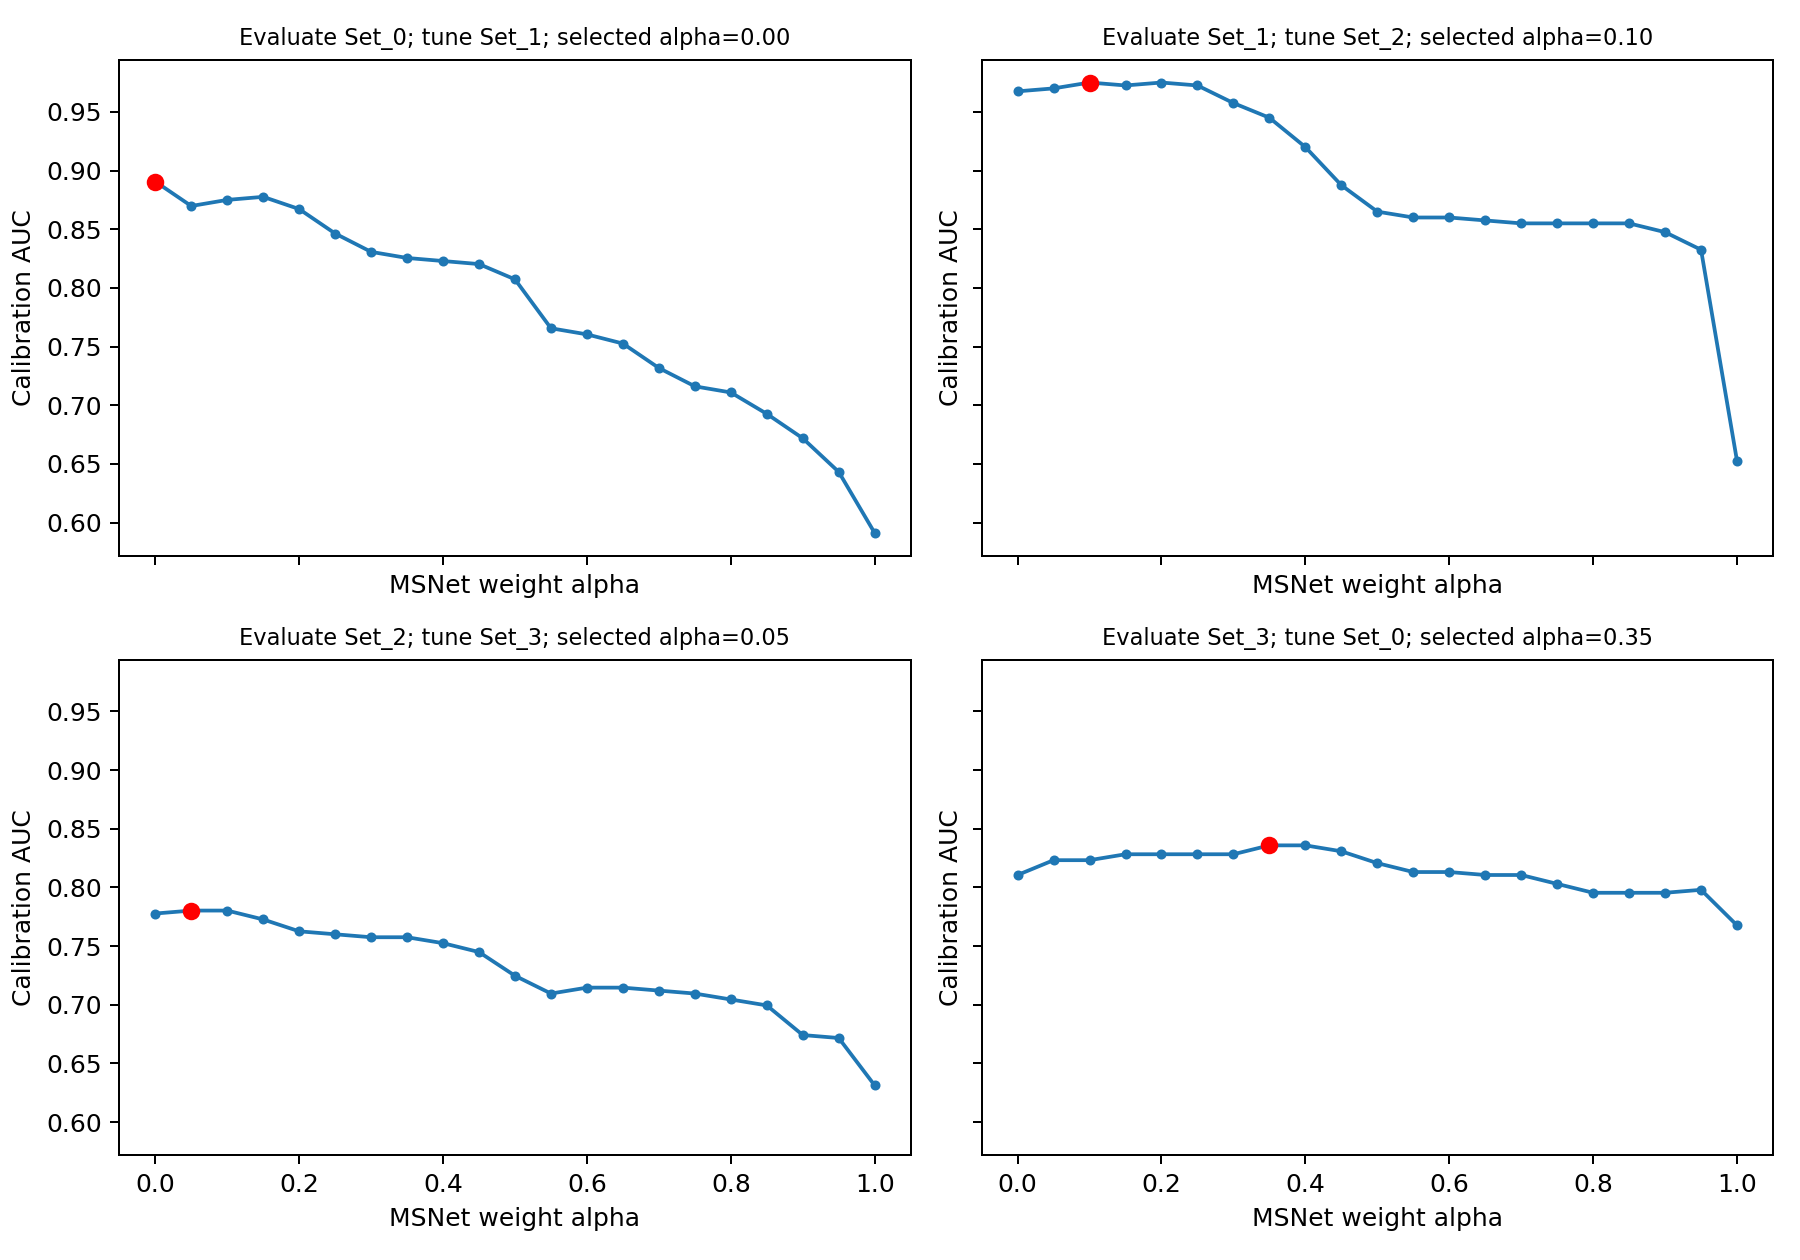
\includegraphics[width=\textwidth]{alpha_calibration_211.png}
\end{center}

\noindent\textbf{Figure S1.} Mean Shift Network (MSNet) weight selection for each EMS fold rotation.
Each panel reports the AUC on the 40 tuning subjects at each weight $\alpha$ in the grid
$\{0,0.05,\ldots,1\}$. The red marker identifies the selected weight.
Selection ranks candidates by AUC, F1-score, and accuracy in that order.
Among candidates still tied, it selects the smallest $\alpha$.
The selected weight and the Otsu threshold computed from the tuning scores are fixed
for the 40 subjects in the evaluation fold.

\medskip
\noindent For the evaluation folds Set\_0 through Set\_3, the selected weights are
$0$, $0.10$, $0.05$, and $0.35$, respectively. A weight of zero uses the behavioral
classifier score alone.

\end{document}
